\chapter{\kadaib}
\section{\purpose}
今回の実験では,反応時間を指標とした視覚探索課題の心理物理実験をする.
心理物理実験とは,物理的世界に属する刺激強度と,心理的世界に属する感覚強度の数学的関数関係を明らかにする実験である\cite{心理物理測定法}.
今回は,視覚探索課題に対して心理物理実験をする.視覚探索課題とは,複数の刺激項目に対して,あらかじめ決められた目標項目があるか否かを,被験者が判断する課題である\cite{視覚探索}.
複数の刺激「妨害刺激」の中に,1つだけ異なる刺激「目標刺激」が存在する場合と,そうでない場合について,刺激数に対する探索時間を結果とする実験を行う.
被験者は,目標刺激が妨害刺激の中にあるかないかを,できるだけ早くかつ正確に判断する必要がある.\par
また,結果に対して統計的仮説検定をする.統計的仮説検定とは,標本を使って母集団に関する統計的な判断を下す方法である\cite[p.200]{Pythonで学ぶあたらしい統計学の教科書}.
今回は\(t\)検定を用いて,視覚探索課題における探索非対称性\footnote{目標刺激と妨害刺激が交代しただけで,探索時間が非常に異なる現象のこと\cite{4視覚探索}.}があるか検討する.仮設は「探索非対称性がある」とし,仮設が正しい場合,目標刺激が異なる2条件に対して回帰直線の傾きに差が生じることを確認する.
\section{\method}
\paragraph{実験装置}
視覚探索課題の心理物理実験には,\matlab とPsychtoolbox を用いる.Psychtoolboxは,プログラミングを簡便にするツールであり,心理物理学の実験でよく用いられる.
データ分析するソフトウェアには\matlab とデータを集計するGoogleスプレットシートを用いる.
\begin{table}[H]
    \caption{実験装置\ (\kadaib)}
    \label{tbl:実験装置\kadaib}
    \begin{tabularx}{\textwidth}{cAR}
        \hline
        \multirow{5}{*}{\bfseries 刺激呈示コンピュータ}  & プロセッサ                    & Intel(R) Xeon(R) Gold 5218R CPU @ 2.10GHz     \\
                                               & メモリ                      & 11.7GB                                        \\
                                               & OS                       & Microsoft Windows 10 Enterprise LTSC 64bit    \\
                                               & \matlab                  & R2020b-academic use                           \\
                                               & Psychtoolbox             & \textbf{◯◯◯◯}                                 \\
        \hline
        \multirow{6}{*}{\bfseries データ分析コンピュータ} & コンピュータ                   & MacBook Air 2022 (Apple社)\texttt{MLY13J/A}    \\
                                               & プロセッサ                    & Apple Silicon M2\ \  8コアCPU,8コアGPU            \\
                                               & メモリ                      & 8GB                                           \\
                                               & OS                       & macOS 13.4                                    \\
                                               & \multirow{2}{*}{\matlab} & R2023a - academic use (Update1 9.14.02239454) \\
                                               &                          & 64-bit (maci64) March 30, 2023                \\
        \hline
    \end{tabularx}
\end{table}
\newpage
\paragraph{視覚探索課題の心理物理実験}
以下に視覚探索課題の心理物理実験方法を示す.

\begin{wrapfigure}{r}[0mm]{.3\textwidth}
    \vspace{-1cm}
    \centering
    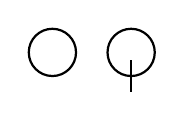
\begin{tikzpicture}
        \draw[thick] (0,0) circle [radius=.3cm];
        \draw[thick] (1,0) circle [radius=.3cm];
        \draw[thick] (1,-.1)--(1,-0.5);
    \end{tikzpicture}
    \caption{刺激対1}
    \label{fig:刺激対1}
    \begin{minipage}[t]{.13\textwidth}
        \centering
        
\includegraphics[keepaspectratio,width=\textwidth]{../../13_BehavioralExperiment/syuri.png}
    \end{minipage}
    \begin{minipage}[t]{.13\textwidth}
        \centering
        
\includegraphics[keepaspectratio,width=\textwidth]{../../13_BehavioralExperiment/star.png}
    \end{minipage}
    \caption{刺激対2}
    \label{fig:刺激対2}
    \vspace{-1cm}
\end{wrapfigure}
\noindent\textbf{\underline{実験1}}
\begin{enumerate}
    \renewcommand{\labelenumi}{\fbox{\theenumi}}
    \item 画面に刺激(刺激対1:\figref{fig:刺激対1})が表示される.画面に表示される合計の刺激数は\(4,8,16\)個のいずれかである.円の刺激を\texttt{C},円と棒の刺激を\texttt{CL}とする.
    \item 目標刺激が妨害刺激の中にある場合は「\texttt{F}」,そうでない場合は「\texttt{J}」を押下する.
    \item 呈示時間は\(500\textrm{ms}\)で,それまでに操作がなければTime overとし,次の刺激を呈示する.
\end{enumerate}
\fbox{1}\ から\ \fbox{3}\ を240回繰り返す.\\
\textbf{\underline{実験2}}\par
ここでは,表示する刺激(刺激対2:\figref{fig:刺激対2})を変更して,同様な実験を行う.左の刺激を\texttt{Star},右の刺激を\texttt{Diamond}とする.
この刺激を選択した理由は,一方の画像に何らかの情報を付加した画像が,もう一方の画像になるからである.
具体的には,\figref{fig:刺激対2}の左図の鋭角を4つから5つに増やす操作をすると,右図の刺激を得られる.
これは\figref{fig:刺激対1}の円に線を付加して得られるもう一方の刺激に習って作成した.
\paragraph{統計的仮説検定}
ここで示す母集団は,調査の対象となる要素の集合.今回の母集団は全人類である.また,母集団の一部を抽出した集合を標本といい,標本に対して検定を行い,母集団の性質を推測する.
\begin{oframed}
    \begin{wrapfigure}{r}[0mm]{.3\textwidth}
        \centering
        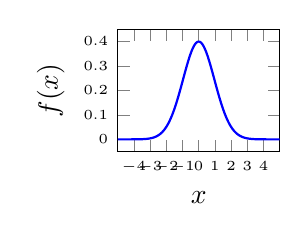
\begin{tikzpicture}
            \begin{axis}
                [
                    width=.3\textwidth,
                    axis lines = box,
                    xmin = -5, xmax = 5, ymin = -0.05, ymax = 0.45,
                    xlabel=\(x\), ylabel=\(f(x)\), samples=300,
                    yticklabel style = {font=\tiny},xticklabel style = {font=\tiny},
                    ytick={0,0.1,0.2,0.3,0.4},
                    yticklabels={0,0.1,0.2,0.3,0.4},
                    xtick={-4,-3,...,4}
                ]
                \addplot[domain=-5:5,thick,blue]{exp(-x^2 / 2) / (sqrt(2*pi) * (1 + x^2)^(1/30))};
            \end{axis}
        \end{tikzpicture}
        \caption{\(t\)分布の確率密度関数(概略)}
        \vspace{-.5cm}
    \end{wrapfigure}
    \noindent\textbf{帰無仮説\ \(H_0\):} 述べたい事柄を否定する仮設.帰無仮説を棄却することで,述べたい事柄を示す.今回は,視覚探索課題において探索非対称性がないことが帰無仮説となる.\\ \\
    \textbf{対立仮設\ \(H_a\):} 述べたい事柄を支持するような仮設を立てる.\\ \\
    \textbf{\(t\)分布:} 正規分布に従う母集団の平均値,分散が不明である場合に利用する確率分布.標本数を\(n\),標本の平均値を\(\bar{X}\),不偏分散を\(s^2\)とし\(t\)分布は\eqref{equ:t分布}で定義される.\(n-1\)の値を自由度と呼び,\(t\)分布は自由度が増すほど正規分布に近づく\cite[p.178\ -\ p.179]{応用解析と情報数学}.
    \begin{align}
        T & =\frac{\bar{X}-\mu}{\sqrt{s^2/n}}\label{equ:t分布}
    \end{align}
    \textbf{\(t\)検定:} \(t\)分布を利用する検定であり,ある値に対して,「ある値と異なる」ことが言えるかどうかを判断する検定方法.ここで用いるある値を\(t\)値とよび,\(t\)値は検定統計量である.今回は自由度を\(n\)としたときの\(t\)値を\eqref{equ:t値}に定める.
    \begin{align}
        t(n) & = \frac{\textrm{回帰直線傾きの平均}}{\textrm{回帰直線傾きの標準誤差}}\label{equ:t値}
    \end{align}
    \textbf{有意確率\ \(p\):} 標本と帰無仮説が矛盾となる目安指標.\(p\)が小さいほど帰無仮説と標本が矛盾している.\\ \\
    \textbf{有意水準\ \(\alpha\):} 帰無仮説を棄却する基準となる値.有意確率\(p\)が有意水準を下回った時に帰無仮説を棄却する.\\ \\
    一般的には\(5\%\)か\(1\%\).今回の実験では,有意水準を\(5\%\)に設定する.
    \begin{itemize}
        \item \(p<\alpha\):有意差があり,帰無仮説が起こる確率が低く帰無仮説を棄却できる.つまり対立仮設を採択できる.
        \item \(p>\alpha\):有意差がなく,帰無仮説が起こる確率を無視できず,帰無仮説を棄却できない.
    \end{itemize}
    \textbf{標準誤差\(\textrm{SE}\):} 理論上の「標本平均の標準偏差」の大きさ.母集団の統計量の誤差を,標本から母集団の性質を推定した統計量の標準偏差として表したもので,\eqref{equ:標準誤差}で求める.
    \begin{align}
        \textrm{SE} & =\frac{\textrm{標準偏差}}{\sqrt{標本サイズ}}\label{equ:標準誤差}
    \end{align}
    \textbf{回帰直線:} 標本\((x_1,y_1),(x_2,y_2),\dots ,(x_n,y_n)\)に対して,
    \begin{align*}
        (y-y_1)^2+(y-y_2)^2+\dots +(y-y_n)^2
    \end{align*}
    を最小にするような直線\(y=ax+b\)を回帰直線という.\\
    \hfill\cite[p.168, p.187, p.200\ -\ p.205]{Pythonで学ぶあたらしい統計学の教科書}
\end{oframed}
データ分析の流れを以下に示す.
\begin{multicols}{2}
    \begin{enumerate}
        \item 帰無仮説,対立仮設を立てる.
        \item 有意水準\(\alpha\)を設定する.
        \item 検定統計量\(t\)値を求める.
        \item \(t\)値から有意確率\(p\)値を求める.
        \item 棄却,採択の判断をする.
              \begin{itemize}
                  \item \(p<\alpha\):帰無仮説を棄却し,対立仮設を採択する.
                  \item \(p>\alpha\):帰無仮説を棄却しない.
              \end{itemize}
        \item \matlab を用いて,データの平均値と標準誤差の誤差線を出力する.
    \end{enumerate}
\end{multicols}
今回の実験では,目標刺激が\texttt{C}と\texttt{CL}それぞれの目標刺激の有無に対して,探索非対称性がないことを帰無仮説とする.
当然,探索非対称性があることが対立仮設となる.データの集計にはGoogleスプレットシートを用いる.以下にGoogleスプレットシート上で用いる関数と,\tblref{tbl:データ集計}に集計方法を示す.
\begin{multicols}{2}
    \begin{description}
        \item[\texttt{AVERAGE(arg)}] 指定範囲の平均.
        \item[\texttt{VAR.S(arg)}] 指定範囲の不偏分散.
        \item[\texttt{STDEV.S(arg)}] 指定範囲の不偏標準偏差(標本標準偏差).
        \item[\texttt{COUNT(arg)}] 指定範囲の要素数.
        \item[\texttt{SQRT(arg)}] 引数の平方根.
        \item[\texttt{TDIST(arg1,arg2,arg3)}] \(p\)値を出力する.\texttt{arg1}には\(t\)値,\texttt{arg2}には自由度\(\textrm{要素数}-1\),\texttt{arg3}には利用確率(今回は両側を利用するので\texttt{2}を代入)を格納する.
        \item[\texttt{SLOPE(arg1,arg2)}] 回帰直線の傾きを出力する.横座標に\texttt{arg1},縦座標に\texttt{arg2}を指定する.
    \end{description}
\end{multicols}
\begin{table}[H]
    \centering
    \caption{Googleスプレットシートを用いたデータ集計}
    \label{tbl:データ集計}
    \begin{tabularx}{\textwidth}{|c|C|C|C|C|C|C|C|C|C|C|C|C|C|C|C|}
        \hline
        \multirow{4}{*}{参加者番号} & \multicolumn{12}{c|}{反応時間}                                                     & \multicolumn{3}{c|}{\multirow{2}{*}{回帰直線の傾き}}                                                                                                                                                                                                                                                                                                                                                                                                                                                                                                                                                                                                                                                                                            \\
        \cline{2-13}
                               & \multicolumn{6}{c|}{Target Type: \texttt{C}}                                   & \multicolumn{6}{c|}{Target type: \texttt{CL}}                  & \multicolumn{3}{c|}{}                                                                                                                                                                                                                                                                                                                                                                                                                                                                                                                                                                                                                                                   \\
        \cline{2-16}
                               & \multicolumn{3}{c|}{Target: YES}                                               & \multicolumn{3}{c|}{Target: NO}                                & \multicolumn{3}{c|}{Target: YES}                               & \multicolumn{3}{c|}{Target: NO} & \multirow{2}{*}{\texttt{C}\footnotemark[1]} & \multirow{2}{*}{\texttt{CL}\footnotemark[1]}                                                             & \multirow{2}{*}{差}                                                                                                                                                                                                                                                                                                                                                                                          \\
        \cline{2-13}
                               & \tikz[remember picture,baseline=(aa.base)]{\node(aa){4}}                       & \tikz[remember picture,baseline=(bb.base)]{\node(bb){8}}       & \tikz[remember picture,baseline=(cc.base)]{\node(cc){16}}      & 4                               & 8                                           & 16                                                                                                       & 4                                                                                                 & 8 & 16 & 4                                                         & 8                                                                              & 16    &                                                                                &  &                                                       \\
        \hline
                               & \tikz[remember picture,baseline=(a0.base)]{\node(a0){}}                        &                                                                &                                                                &                                 &                                             &                                                                                                          &                                                                                                   &   &    &                                                           &                                                                                &       &                                                                                &  & \tikz[remember picture,baseline=(m.base)]{\node(m){}} \\
                               & \tikz[remember picture,baseline=(a1.base)]{\node(a1){\(a_1\)}}                 & \tikz[remember picture,baseline=(a2.base)]{\node(a2){\(a_2\)}} & \tikz[remember picture,baseline=(a3.base)]{\node(a3){\(a_3\)}} &                                 &                                             &                                                                                                          &                                                                                                   &   &    & \multicolumn{3}{r|}{\texttt{SLOPE(a,NoT)}\(\rightarrow\)} & \(m\)                                                                          & \(n\) & {\tiny\(m-n\)}                                                                                                                            \\
                               &                                                                                &                                                                &                                                                &                                 &                                             &                                                                                                          &                                                                                                   &   &    &                                                           &                                                                                &       &                                                                                &  &                                                       \\
                               & \tikz[remember picture,baseline=(a4.base)]{\node(a4){}}                        &                                                                &                                                                &                                 &                                             &                                                                                                          &                                                                                                   &   &    &                                                           &                                                                                &       &                                                                                &  & \tikz[remember picture,baseline=(n.base)]{\node(n){}} \\
        \hline
        {\small 平均値}           & \tikz[remember picture,baseline=(w1.base)]{\node(w1){\scriptsize\texttt{AVE}}} &                                                                &                                                                &                                 &                                             &                                                                                                          & \multicolumn{3}{c|}{\tikz[remember picture,baseline=(w.base)]{\node(w){\texttt{AVERAGE(range)}}}} &   &    &                                                           &                                                                                &       & \tikz[remember picture,baseline=(w2.base)]{\node(w2){\tiny\texttt{sAVE}}}                                                                 \\
        \hline
        不偏分散                   & \tikz[remember picture,baseline=(x1.base)]{\node(x1){\scriptsize\texttt{UV}}}  &                                                                &                                                                &                                 &                                             &                                                                                                          & \multicolumn{3}{c|}{\tikz[remember picture,baseline=(x.base)]{\node(x){\texttt{VAR.S(range)}}}}   &   &    &                                                           &                                                                                &       & \tikz[remember picture,baseline=(x2.base)]{\node(x2){\scriptsize\texttt{sUV}}}                                                            \\
        \hline
        標準偏差                   & \tikz[remember picture,baseline=(y1.base)]{\node(y1){\scriptsize\texttt{SD}}}  &                                                                &                                                                &                                 &                                             &                                                                                                          & \multicolumn{3}{c|}{\tikz[remember picture,baseline=(y.base)]{\node(y){\texttt{AVERAGE(range)}}}} &   &    &                                                           &                                                                                &       & \tikz[remember picture,baseline=(y2.base)]{\node(y2){\scriptsize\texttt{sSD}}}                                                            \\
        \hline
        標準誤差                   & \tikz[remember picture,baseline=(z1.base)]{\node(z1){\scriptsize\texttt{SE}}}  &                                                                &                                                                &                                 &                                             & \multicolumn{5}{c|}{\tikz[remember picture,baseline=(z.base)]{\node(z){\texttt{SD/SQRT(COUNT(range))}}}} &                                                                                                   &   &    &                                                           & \tikz[remember picture,baseline=(z2.base)]{\node(z2){\scriptsize\texttt{sSE}}}                                                                                                                                                     \\
        \hline
    \end{tabularx}
\end{table}
\begin{tikzpicture}[remember picture,overlay]
    \node[inner xsep=1.5em,inner ysep=1mm,fit={(aa.base)(bb)(cc.base)},thick,fill=red,fill opacity=0.2](wrap_ind){};
    \node[inner xsep=1.5em,inner ysep=1mm,fit={(a1.base)(a2)(a3.base)},thick,fill=blue,fill opacity=0.2](wrap_ind2){};
    \node[inner xsep=1em,inner ysep=.7mm,fit={(a0)(a4)},thick,very thick,rounded corners,draw](wrap_ind3){};
    \node[inner xsep=1em,inner ysep=.7mm,fit={(m)(n)},thick,very thick,rounded corners,draw](wrap_ind4){};
    \node[below left=.5cm of wrap_ind](ind){\texttt{NoT}};
    \node[below right=.5cm of wrap_ind2](ind2){\texttt{a}};
    \node[below right=.35cm of wrap_ind3.east,fill=white](ind3){\texttt{range}};
    \node[below left=.35cm of wrap_ind4.west,fill=white](ind4){\texttt{range\_s}};
    \draw[-latex](ind.north east)--(wrap_ind.south west);
    \draw[-latex](ind2.north west)--(wrap_ind2.south east);
    \draw[-latex](ind3.west)--(wrap_ind3.east |- ind3.west);
    \draw[-latex](ind4.east)--(wrap_ind4.west |- ind3.east);
    \foreach \u in{w,x,y,z}{
            \draw[dotted,-latex,line width=6pt,white](\u)--(\u 1);
            \draw[dotted,-latex,line width=6pt,white](\u)--(\u 2);
            \draw[thick,dotted,-latex](\u)--(\u 1);
            \draw[thick,dotted,-latex](\u)--(\u 2);
        }
\end{tikzpicture}
\footnotetext[1]{目標刺激の種類}
\(t\)値を\texttt{t = sAVE/sSD},\(p\)値を\texttt{p = TDIST(t,COUNT(range\_s)-1,2)}で求め,\tblref{tbl:データ集計}を\csv 形式で書き出す.\par
次に,\matlab でデータの平均値と標準誤差の誤差線を出力するスクリプトを記述する.\texttt{importdata}関数を用いて書き出した\csv を読み込む.
参加者番号を削除した後に,各統計量を求める.そのデータから平均値と標準誤差の誤差線を\texttt{err\_data}関数を用いて描画する.\par
最後に,読み込んだデータから回帰直線を求める.\tblref{tbl:データ集計}に示した方法を\matlab で再現し,\texttt{polyfit}関数と\texttt{slope}関数を用いて回帰直線の傾きと切片を求める.
自分自身のデータを散布図として,回帰直線と同時に描画する.
\section{\result}
刺激(\figref{fig:刺激対1},\figref{fig:刺激対2})の,刺激数に対する反応時間を示したグラフを\figref{fig:刺激対の刺激数に対する反応時間}に示す.
被験者集団\(A\)の平均値と標準誤差の誤差線を\figref{fig:平均値と誤差線},その回帰線を\figref{fig:平均値と回帰直線}に示す.
グラフ作成のもととなったデータを\tblref{tbl:反応時間},\tblref{tbl:回帰直線の傾き}に示す.
\begin{figure}[H]
    \centering
    \begin{minipage}[b]{.49\textwidth}
        \centering
        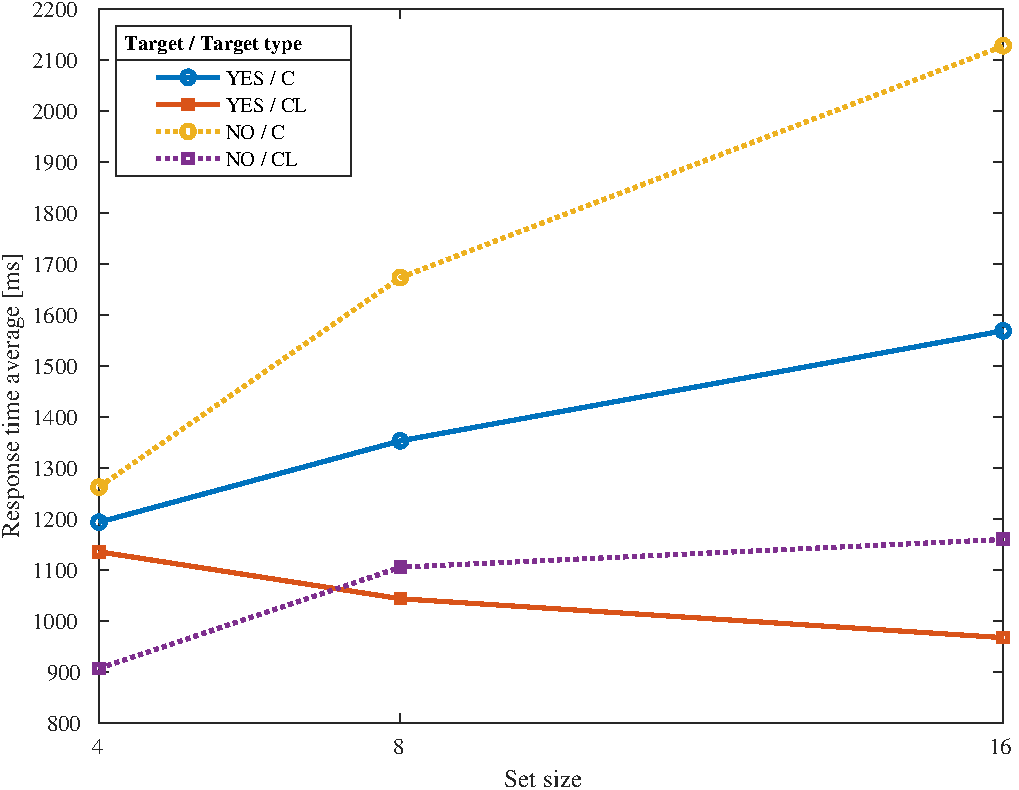
\includegraphics[keepaspectratio,width=\textwidth]{../../Figures/13_01_graph.pdf}
        \subcaption{刺激対1の刺激数に対する反応時間}
    \end{minipage}
    \begin{minipage}[b]{.49\textwidth}
        \centering
        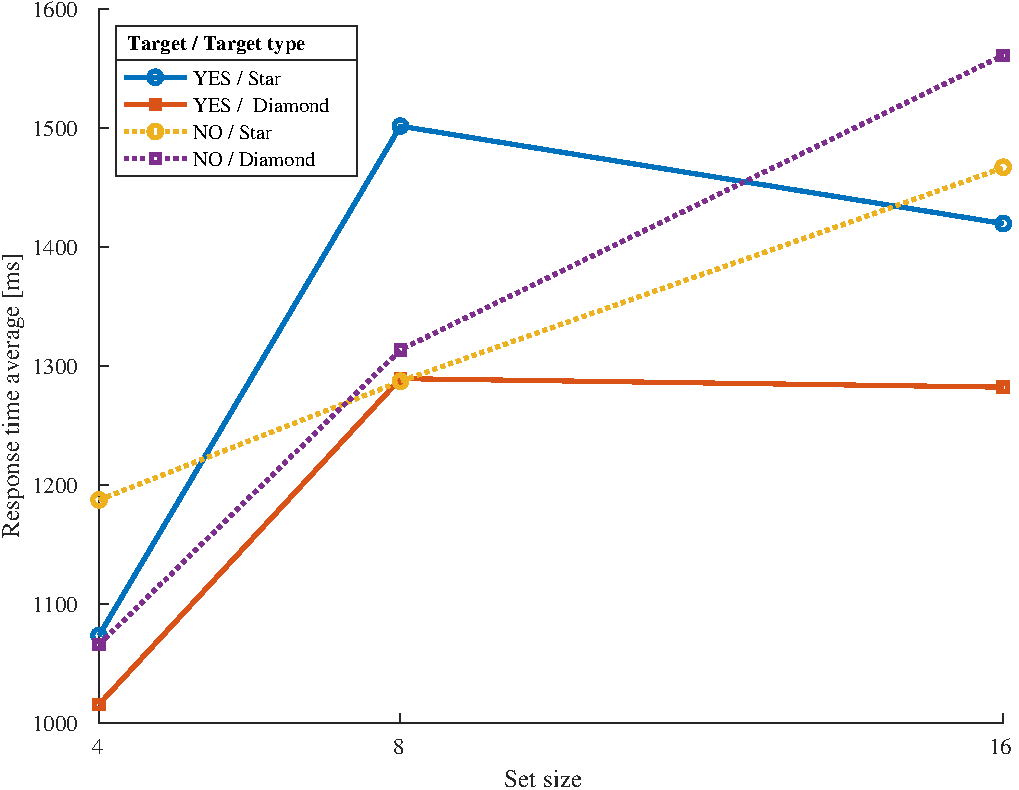
\includegraphics[keepaspectratio,width=\textwidth]{../../Figures/13_02_graph.pdf}
        \subcaption{刺激対2の刺激数に対する反応時間}
    \end{minipage}
    \caption{刺激に対する反応時間}
    \label{fig:刺激対の刺激数に対する反応時間}
\end{figure}
\begin{figure}[H]
    \centering
    \begin{minipage}[b]{.49\textwidth}
        \centering
        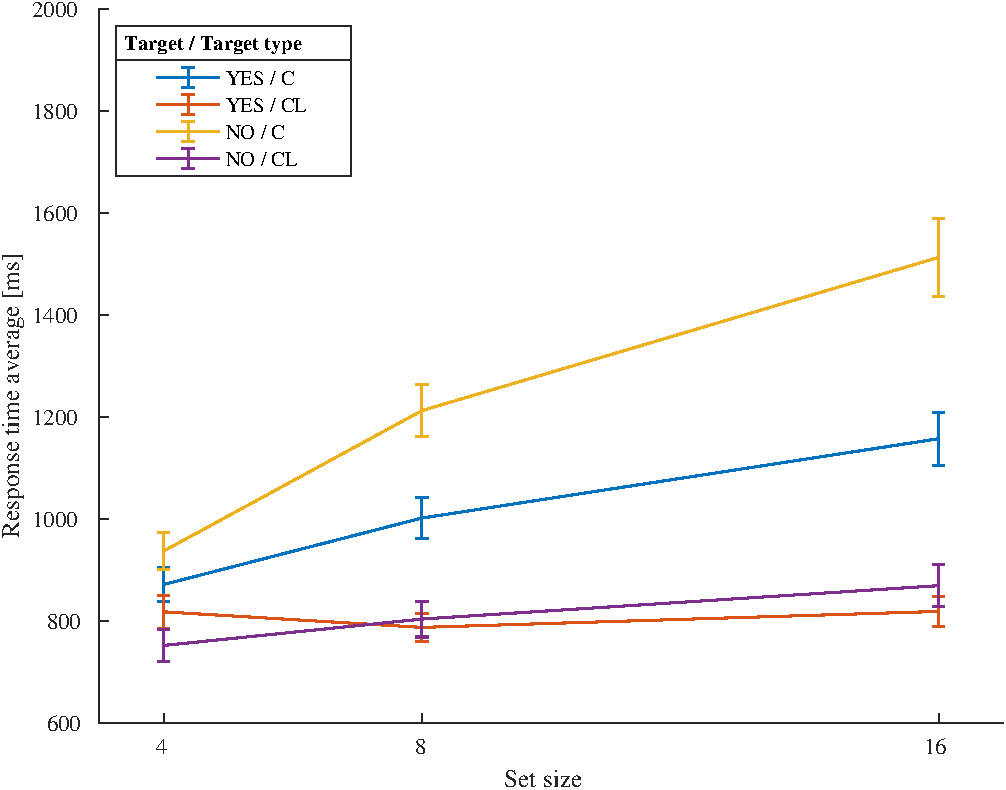
\includegraphics[keepaspectratio,width=\textwidth]{../../Figures/14_01_graph.pdf}
        \caption{平均値と誤差線}
        \label{fig:平均値と誤差線}
    \end{minipage}
    \begin{minipage}[b]{.49\textwidth}
        \centering
        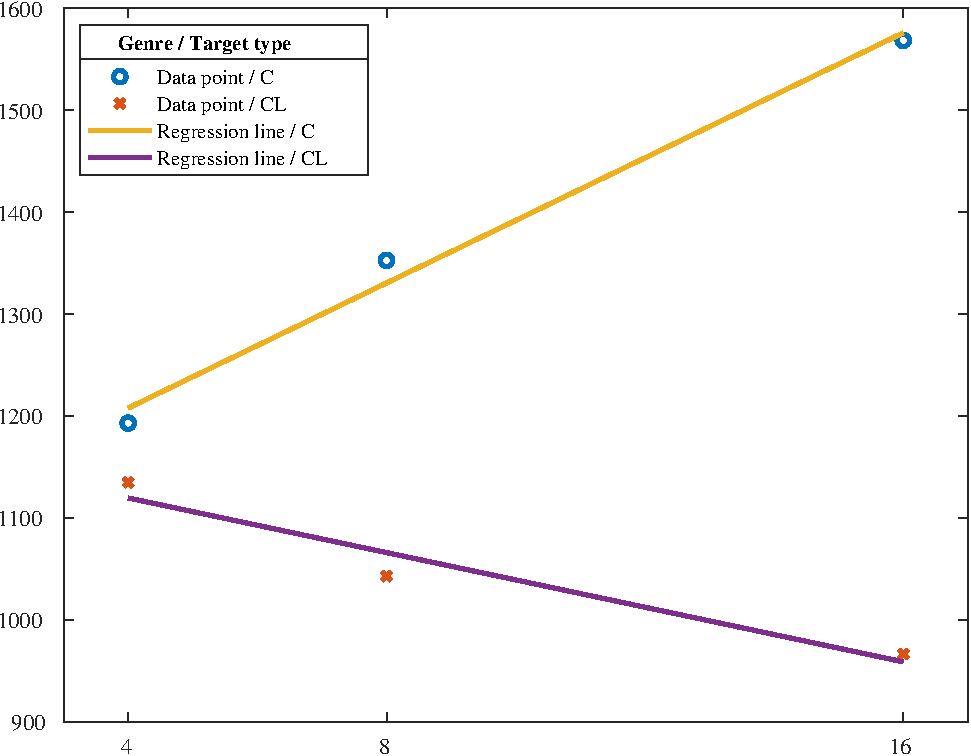
\includegraphics[keepaspectratio,width=\textwidth]{../../Figures/14_02_graph.pdf}
        \caption{平均値と回帰直線}
        \label{fig:平均値と回帰直線}
    \end{minipage}
\end{figure}
有意水準\(5\%\)で対応のある\(t\)検定を行った結果,刺激対1の刺激\texttt{C}と\texttt{CL}の間で有意な差が認められた.
\begin{align}
    t(13) & =2.9150238 & p<0.05
\end{align}
\begin{table}[H]
    \centering
    \caption{反応時間}
    \label{tbl:反応時間}
    \fontsize{4}{3}\selectfont\ttfamily
    \begin{tabularx}{\textwidth}{|c|L|L|L|L|L|L|L|L|L|L|L|L|}
    \hline
    \multirow{3}{*}{ID} & \multicolumn{6}{c|}{目標刺激:円}  & \multicolumn{6}{c|}{目標刺激:円+線}                                                                                                                                                                                 \\
    \cline{2-13}
                        & \multicolumn{3}{c|}{目標刺激:あり} & \multicolumn{3}{c|}{目標刺激:なし}  & \multicolumn{3}{c|}{目標刺激: あり} & \multicolumn{3}{c|}{目標刺激: なし}                                                                                                                 \\
    \cline{2-13}
                        & 4                            & 8                             & 16                            & 4                             & 8           & 16          & 4           & 8           & 16          & 4           & 8           & 16          \\
    \hline
    非表示                 & 783.105                      & 872                           & 980.867                       & 857.2                         & 1042.63     & 1338.65     & 768.222     & 761.389     & 750.778     & 710.65      & 754.579     & 811.5       \\ \hline
    非表示                 & 1193.17                      & 1352.79                       & 1568.67                       & 1262.2                        & 1673.22     & 2128.1      & 1135.1      & 1043.06     & 966.65      & 906.4       & 1104.85     & 1159.75     \\ \hline
    非表示                 & 698                          & 979                           & 984.143                       & 791.25                        & 1089.35     & 1199.75     & 651.211     & 621.688     & 656.412     & 598.722     & 594.947     & 684.737     \\ \hline
    非表示                 & 888.421                      & 1061.72                       & 1314.4                        & 925.526                       & 1025.88     & 1095.28     & 888.421     & 923.2       & 1081        & 845.611     & 842.947     & 809.842     \\ \hline
    非表示                 & 878.778                      & 963.158                       & 1236.47                       & 908.7                         & 1239        & 1619.55     & 866.389     & 747.263     & 838.471     & 652.05      & 744.2       & 872.7       \\ \hline
    非表示                 & 849.632                      & 848                           & 994.167                       & 738.105                       & 1079.79     & 1214        & 681.75      & 721.765     & 703.158     & 624.611     & 695         & 716.947     \\ \hline
    非表示                 & 755.95                       & 943.105                       & 1037.67                       & 845.053                       & 1053.65     & 1339.16     & 745.556     & 807.389     & 781.316     & 677.526     & 737.25      & 722.278     \\ \hline
    非表示                 & 922.5                        & 898.895                       & 1104.83                       & 867.15                        & 1116.9      & 1424.55     & 835.8       & 882         & 822.278     & 714.4       & 790.9       & 744.526     \\ \hline
    非表示                 & 913.824                      & 1187.14                       & 1283.6                        & 1049.47                       & 1273.67     & 1442.74     & 961.737     & 802.95      & 857.1       & 842.444     & 790.333     & 890.05      \\ \hline
    非表示                 & 776.95                       & 926.526                       & 1023.68                       & 926                           & 1198.58     & 1756.15     & 747.263     & 724.895     & 738.263     & 613.053     & 646.7       & 755.15      \\ \hline
    非表示                 & 862.158                      & 966.056                       & 1141.71                       & 890.053                       & 1237        & 1666.6      & 821.368     & 704.5       & 747.4211    & 808.2       & 812.294     & 831.579     \\ \hline
    非表示                 & 1000.21                      & 1182                          & 1244.66                       & 1006                          & 1423.25     & 1679.35     & 800.8       & 788.75      & 826.3       & 806.26      & 834.05      & 941.75      \\ \hline
    非表示                 & 814.25                       & 990.25                        & 1354.11                       & 1131                          & 1459.3      & 1841.15     & 761.55      & 764.95      & 840.05      & 718.15      & 810.8       & 1017.6      \\ \hline
    非表示                 & 909.278                      & 1001.76                       & 1238.6                        & 914                           & 1057.85     & 1433.95     & 777.74      & 721.333     & 844.579     & 946.438     & 931.944     & 892.667     \\ \hline\hline
    平均値                 & 874.7304286                  & 1012.314286                   & 1179.112643                   & 936.5505                      & 1212.147857 & 1512.784286 & 817.3505    & 786.7951429 & 818.1268643 & 747.4653571 & 792.1995714 & 846.5054286 \\ \hline
    不偏分散                & 14623.15518                  & 19668.22447                   & 29640.45678                   & 18852.99019                   & 36736.541   & 80724.11463 & 14850.098   & 11007.30814 & 11615.11971 & 12556.73028 & 15278.89779 & 17008.08359 \\ \hline
    標準偏差                & 120.9262386                  & 140.2434472                   & 172.1640403                   & 137.3061914                   & 191.6677881 & 284.1198948 & 121.8609782 & 104.9157192 & 107.7734648 & 112.0568172 & 123.6078387 & 130.4150436 \\ \hline
    標準誤差                & 32.31889671                  & 38.89653383                   & 47.74971348                   & 38.08188565                   & 53.15907984 & 78.8006807  & 33.79815425 & 29.09838502 & 29.89098103 & 31.07896925 & 34.28264619 & 36.17062513 \\ \hline
\end{tabularx}

\end{table}
\begin{table}[H]
    \centering
    \caption{回帰直線の傾き}
    \label{tbl:回帰直線の傾き}
    \fontsize{4}{1}\selectfont\ttfamily
    \begin{tabularx}{\textwidth}{|c|L|L|L|}
    \hline
    参加者番号                  & \multicolumn{1}{c|}{目標刺激:円} & \multicolumn{1}{c|}{目標刺激:円+線} & \multicolumn{1}{c|}{差} \\
    \hline
    非表示                    & 16.06991071                 & -1.435482143                  & 17.50539286            \\ \hline
    {\normalfont 参加者\(A\)} & 30.67642857                 & -13.39660714                  & 44.07303571            \\ \hline
    非表示                    & 20.530625                   & 0.9915714286                  & 19.53905357            \\ \hline
    非表示                    & 34.93921429                 & 16.5735                       & 18.36571429            \\ \hline
    非表示                    & 30.43                       & -0.3654285714                 & 30.79542857            \\ \hline
    非表示                    & 12.93405357                 & 1.196875                      & 11.73717857            \\ \hline
    非表示                    & 16.70098214                 & -2.032321429                  & 18.73330357            \\ \hline
    非表示                    & 28.13507143                 & -6.507107143                  & 34.64217857            \\ \hline
    非表示                    & 19.35846429                 & -0.4041428571                 & 19.76260714            \\ \hline
    非表示                    & 21.81151786                 & 2.088696429                   & 19.72282143            \\ \hline
    非表示                    & 23.10467857                 & -4.515473214                  & 27.62015179            \\ \hline
    非表示                    & 45.05892857                 & 6.948214286                   & 38.11071429            \\ \hline
    非表示                    & 27.75228571                 & 6.975035714                   & 20.77725               \\ \hline
    非表示                    & 18.57964286                 & 2.491964286                   & 16.08767857            \\ \hline\hline
    平均値                    & 24.72012883                 & 0.6149496173                  & 24.10517921            \\ \hline
    不偏分散                   & 75.39627981                 & 48.30711698                   & 88.89262924            \\ \hline
    標準偏差                   & 8.683103121                 & 6.950332149                   & 9.428288776            \\ \hline
    標準誤差                   & 2.320656924                 & 1.857554402                   & 2.519816167            \\ \hline
\end{tabularx}
\end{table}
